\section{Cơ sở thiết kế trò chơi}
\subsection{Tổng quan trò chơi}
\hspace*{1cm} \textbf{MeowSQL Knight} là một trò chơi nhập vai Phiêu lưu chiến đấu theo lượt. Thay vì sử dụng các thao tác thông thường bằng các nút, người chơi tương tác bằng các nhập câu truy vấn và thực thi chúng, thu thập dữ kiện để chiếm lấy ưu thế trong chiến đấu, đánh bại quái vật và hoàn thành màn chơi.\\
\begin{figure}[H]
	\centering
	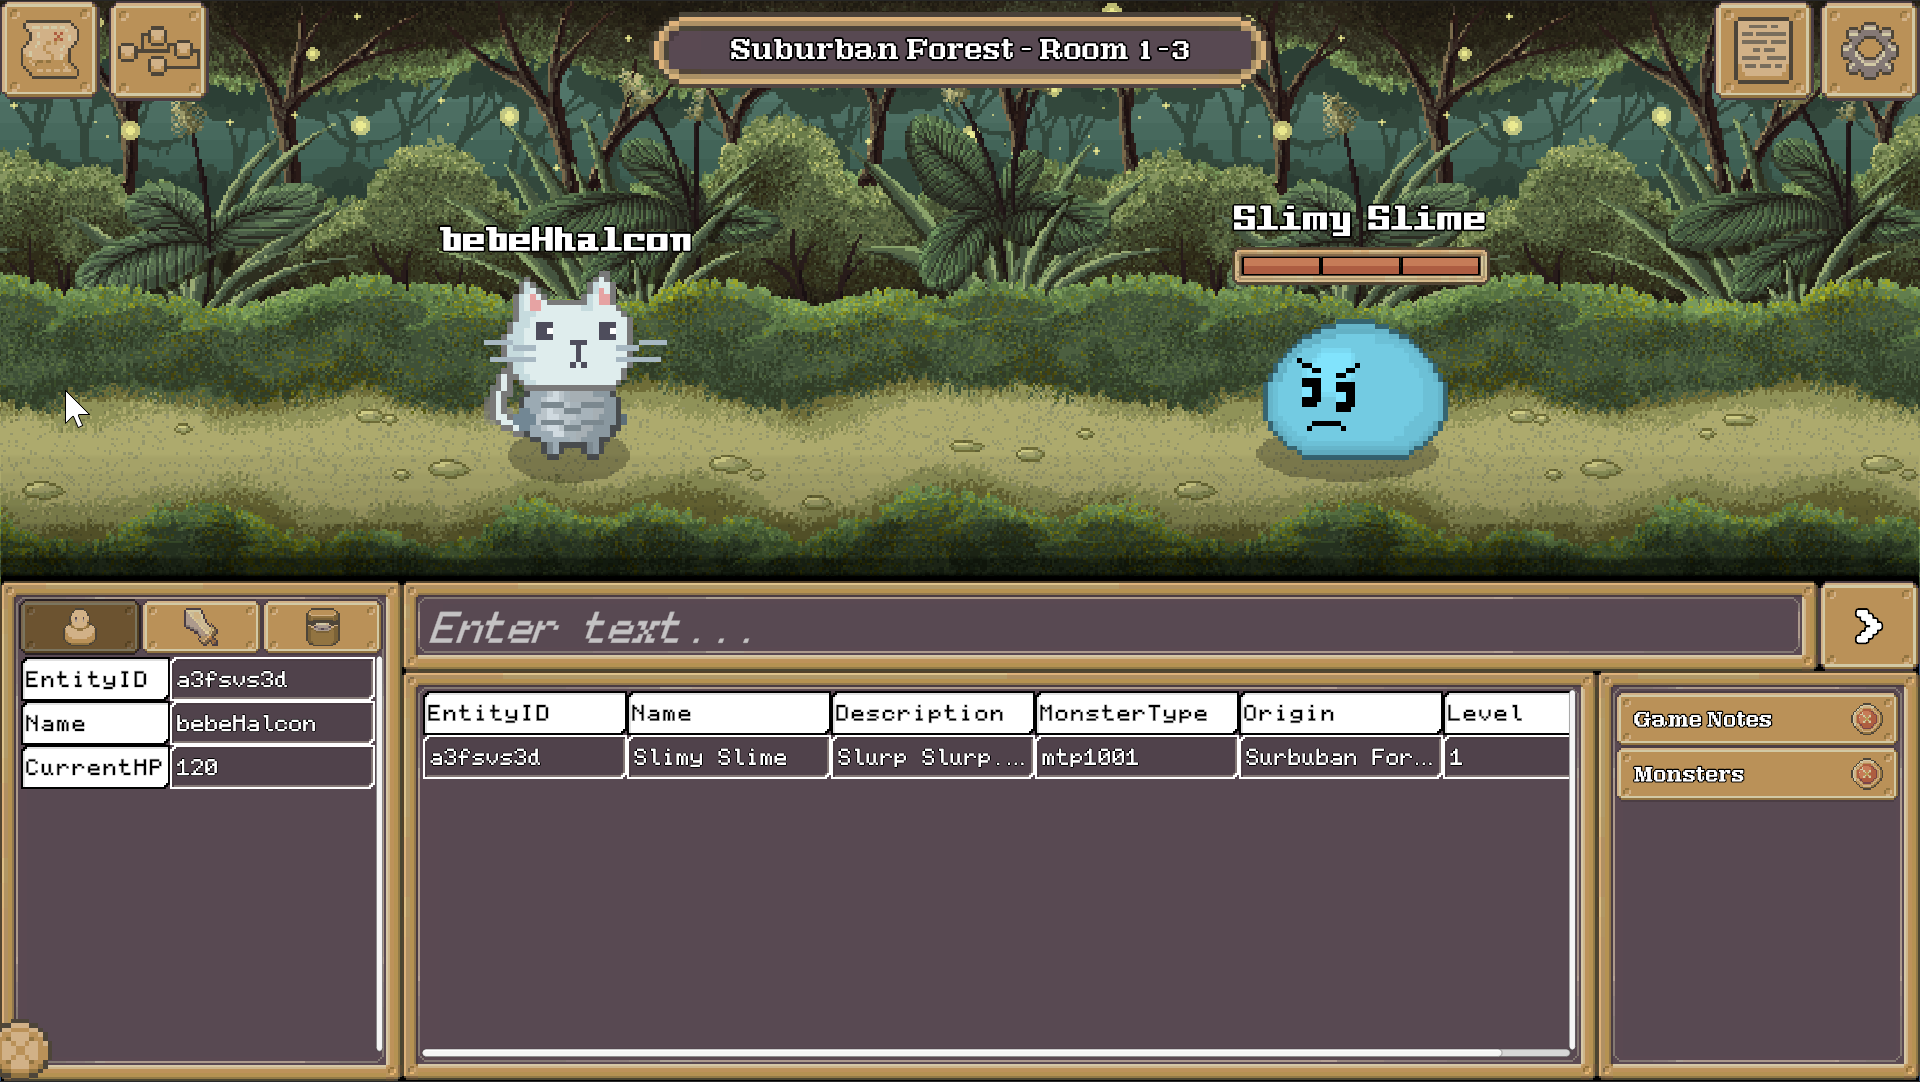
\includegraphics[width=\textwidth]{Images/Overall.png}
	\vspace{0.5cm}
	\caption{Tổng quan một màn chơi trong MeowSQL Knight}
\end{figure}
\hspace*{1cm} Người chơi sẽ sử dụng các câu truy vấn để khai thác schema cho sẵn. Sử dụng \textbf{select} để hiện nội dung các record lên màn hình, thu thập thông tin từ những dữ liệu đó. Ngoài ra cũng có thể \textbf{insert} và \textbf{delete} những record trên bảng và xem phản ứng của trò chơi sẽ như thế nào. Người chơi sẽ tấn công quái vật bằng các vũ khí mà người chơi mang vào trận chiến, tuy nhiên không thể tấn công quái vật một cách đơn thuần, người chơi sẽ phải tấn công vào các điểm yếu của quái vật nằm trên các bộ phận khác nhau. Để tương tác với game (tấn công quái vật, dùng vật phẩm), người chơi sẽ insert các tham số vào các bảng có chức năng đặc biệt, sau khi chèn xong thì hành động sẽ được thực thi.\\
\hspace*{1cm} Trong Schema này, các thực thể như người chơi, quái vật, bộ phận chí mạng của quái vật,... đều sử dụng chung ID có cấu trúc như nhau. Để tiêu diệt quái vật, người chơi phải nhắm đến các bộ phận chí mạng này, cũng như xác định được ID của chúng để có thể tấn công chính xác, bằng không các đòn đánh của người chơi sẽ bị trượt.\\
\hspace*{1cm} Người chơi phải tìm cách khai thác schema một cách hiệu quả trong chiến đấu. Đi kèm với việc lựa chọn trang bị hợp lý và tận dụng lợi thế môi trường, giành chiến thắng, hoàn thành màn chơi và đi sâu hơn để tìm ra bí ẩn của trò chơi.


\subsection{Sơ lược cốt truyện}
\hspace*{1cm} Trong một thế giới game RPG có chủ đề là động vật bình thường, bạn là một kỵ sĩ mèo đang đi rừng để tìm nguyên liệu, mọi thứ diễn ra một cách bình thường. \\
\hspace*{1cm} Đột nhiên, trò chơi bỗng hoạt động không đúng so với trước kia, các quái vật trở nên hung hãn hơn, nguy hiểm hơn, lẽ ra chỉ cần đánh bằng các phương pháp thông thường đã có thể diệt sạch chúng, nhưng kì lạ thay, các phương pháp thông thường không còn có hiệu quả với chúng nữa. Đám quái vật vùng lên làm loạn cả thế giới game, khiến thế giới game bị lỗi nghiêm trọng, và nếu cứ tiếp tục như vậy, trò chơi sẽ không thể chơi được nữa.\\
\hspace*{1cm} Chính lúc này, nhân vật chính của chúng ta bị một con slime bao vây, lẽ ra 1 nhát từ kiếm của cậu có thể hạ gục con Slime, tuy nhiên, trong thế giới game bị rối loạn như thế này là không thể. Cậu cứ đánh trong vô vọng, trong khi con quái vật giận dữ tiến gần định nuốt chửng cậu. Đột nhiên, một tia sáng xuất hiện giết chết con quái vật đó. Là Nhà phát triển (Dev) của trò chơi này. Anh ấy đã kiểm tra hệ thống thế giới game và phát hiện ra bạn là một trong những object hiếm hoi còn sống trong thế giới game này. Để hỗ trợ bạn, Dev cấp cho bạn 1 năng lực lớn: bạn có thể xem schema của game và thực hiện các câu truy vấn SQL để khai thác schema và chiến đấu. Vì chỉ có sử dụng SQL mới có thể đánh bại các quái vật SQL. \\
\hspace*{1cm} Dev muốn đặt niềm tin vào bạn vì Dev không thể khởi dộng lại Project game này, nó là một project chạy trên server nhưng cậu đã mất quyền kiểm soát cả server và project. Dev muốn bạn đi sâu vào bên trong lõi của game và tìm ra lý do khiến game trở nên như vậy. Bạn là hy vọng của thế giới game này, và là hy vọng của cả Dev. Bạn bắt đầu đi vào sâu trong thế giới, mang sứ mệnh vô cùng cao cả, không chỉ để cứu thế giới này.

\subsection{So Sánh các sản phẩm tương tự trên thị trường}
\hspace*{1cm} Nhắc đến dòng game giải đố theo lượt chúng ta không thể bỏ qua series game \textbf{Bookworm Adventures} được phát triển bởi \textit{\textbf{PopCap Games}}. Đây là một trong những trò chơi độc đáo kết hợp giữa ghép chữ và chiến đấu theo lượt, tạo ra phong cách riêng biệt và mới mẻ trong dòng game này.\\
\hspace*{1cm} Ở thời điểm hiện tại, trò chơi giải đố dựa trên cấu trúc của ngôn ngữ lập trình SQL đã xuất hiện trong một số sản phẩm. Sản phẩm nổi bật nhất là \textbf{SQL Murder Mystery} được phát triển bởi \textit{\textbf{Knight Lab}} của Đại học Northwestern, Mỹ.
\begin{figure}[H]
\centering
\begin{minipage}{.5\textwidth}
  \centering
  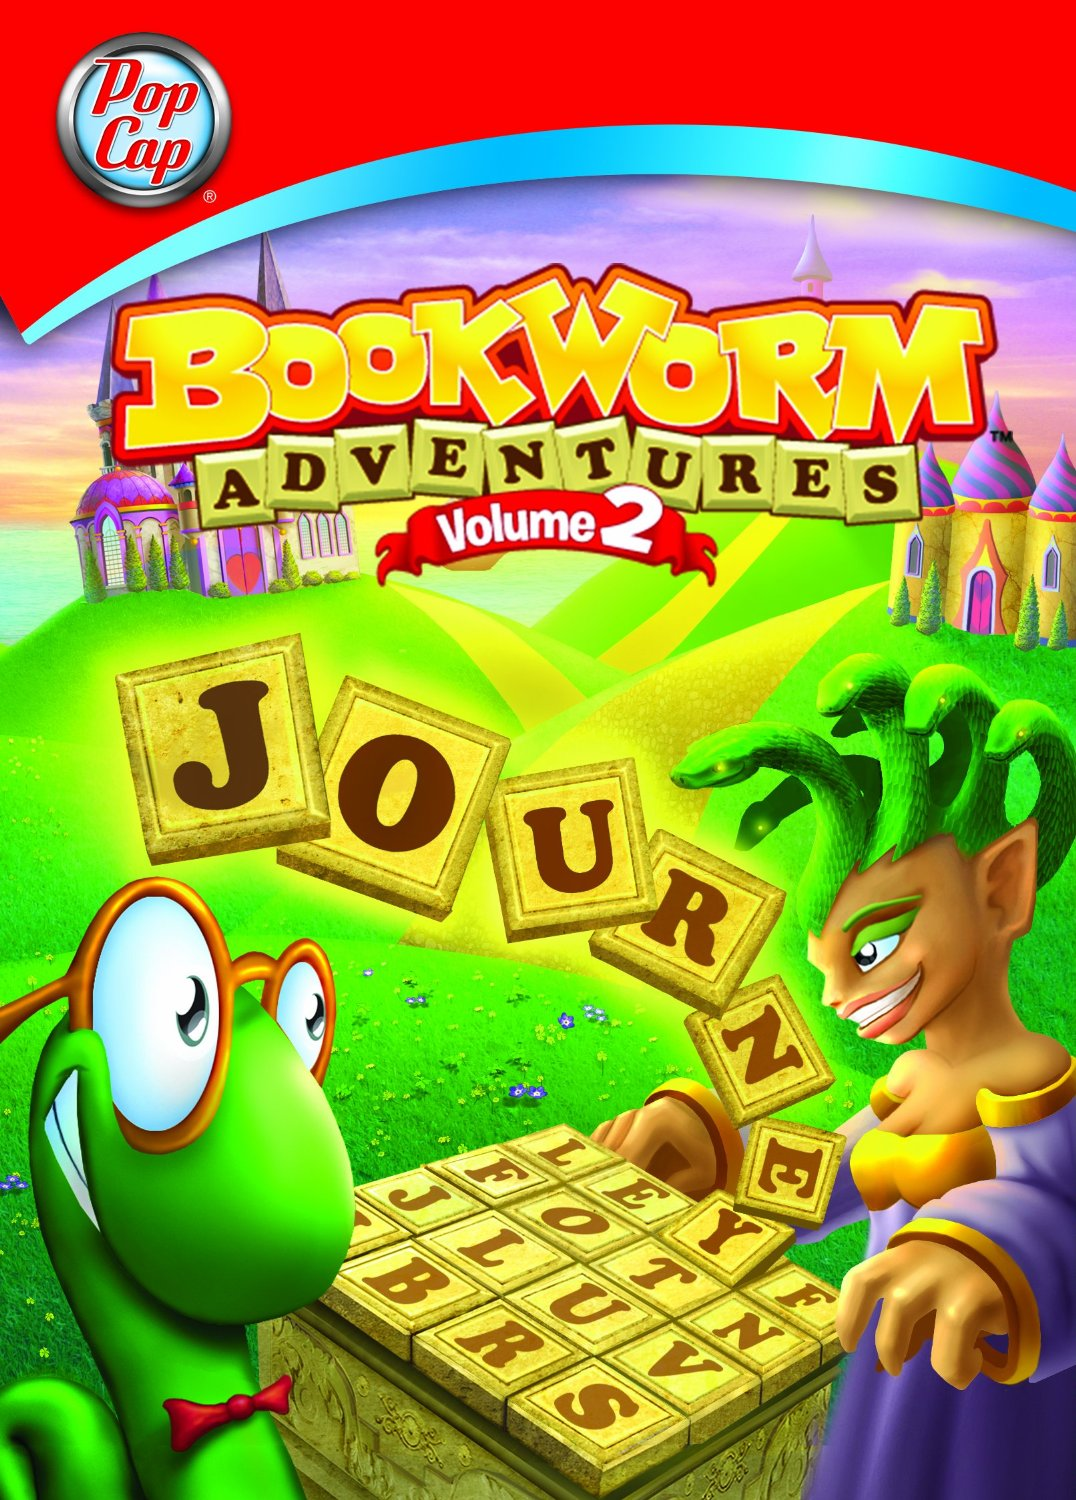
\includegraphics[width=.5\linewidth]{Images/bookworm.jpg}
  \vspace{0.5cm}
  \caption{Bookworm Adventures}
  \label{fig:test1}
\end{minipage}%
\begin{minipage}{.5\textwidth}
  \centering
  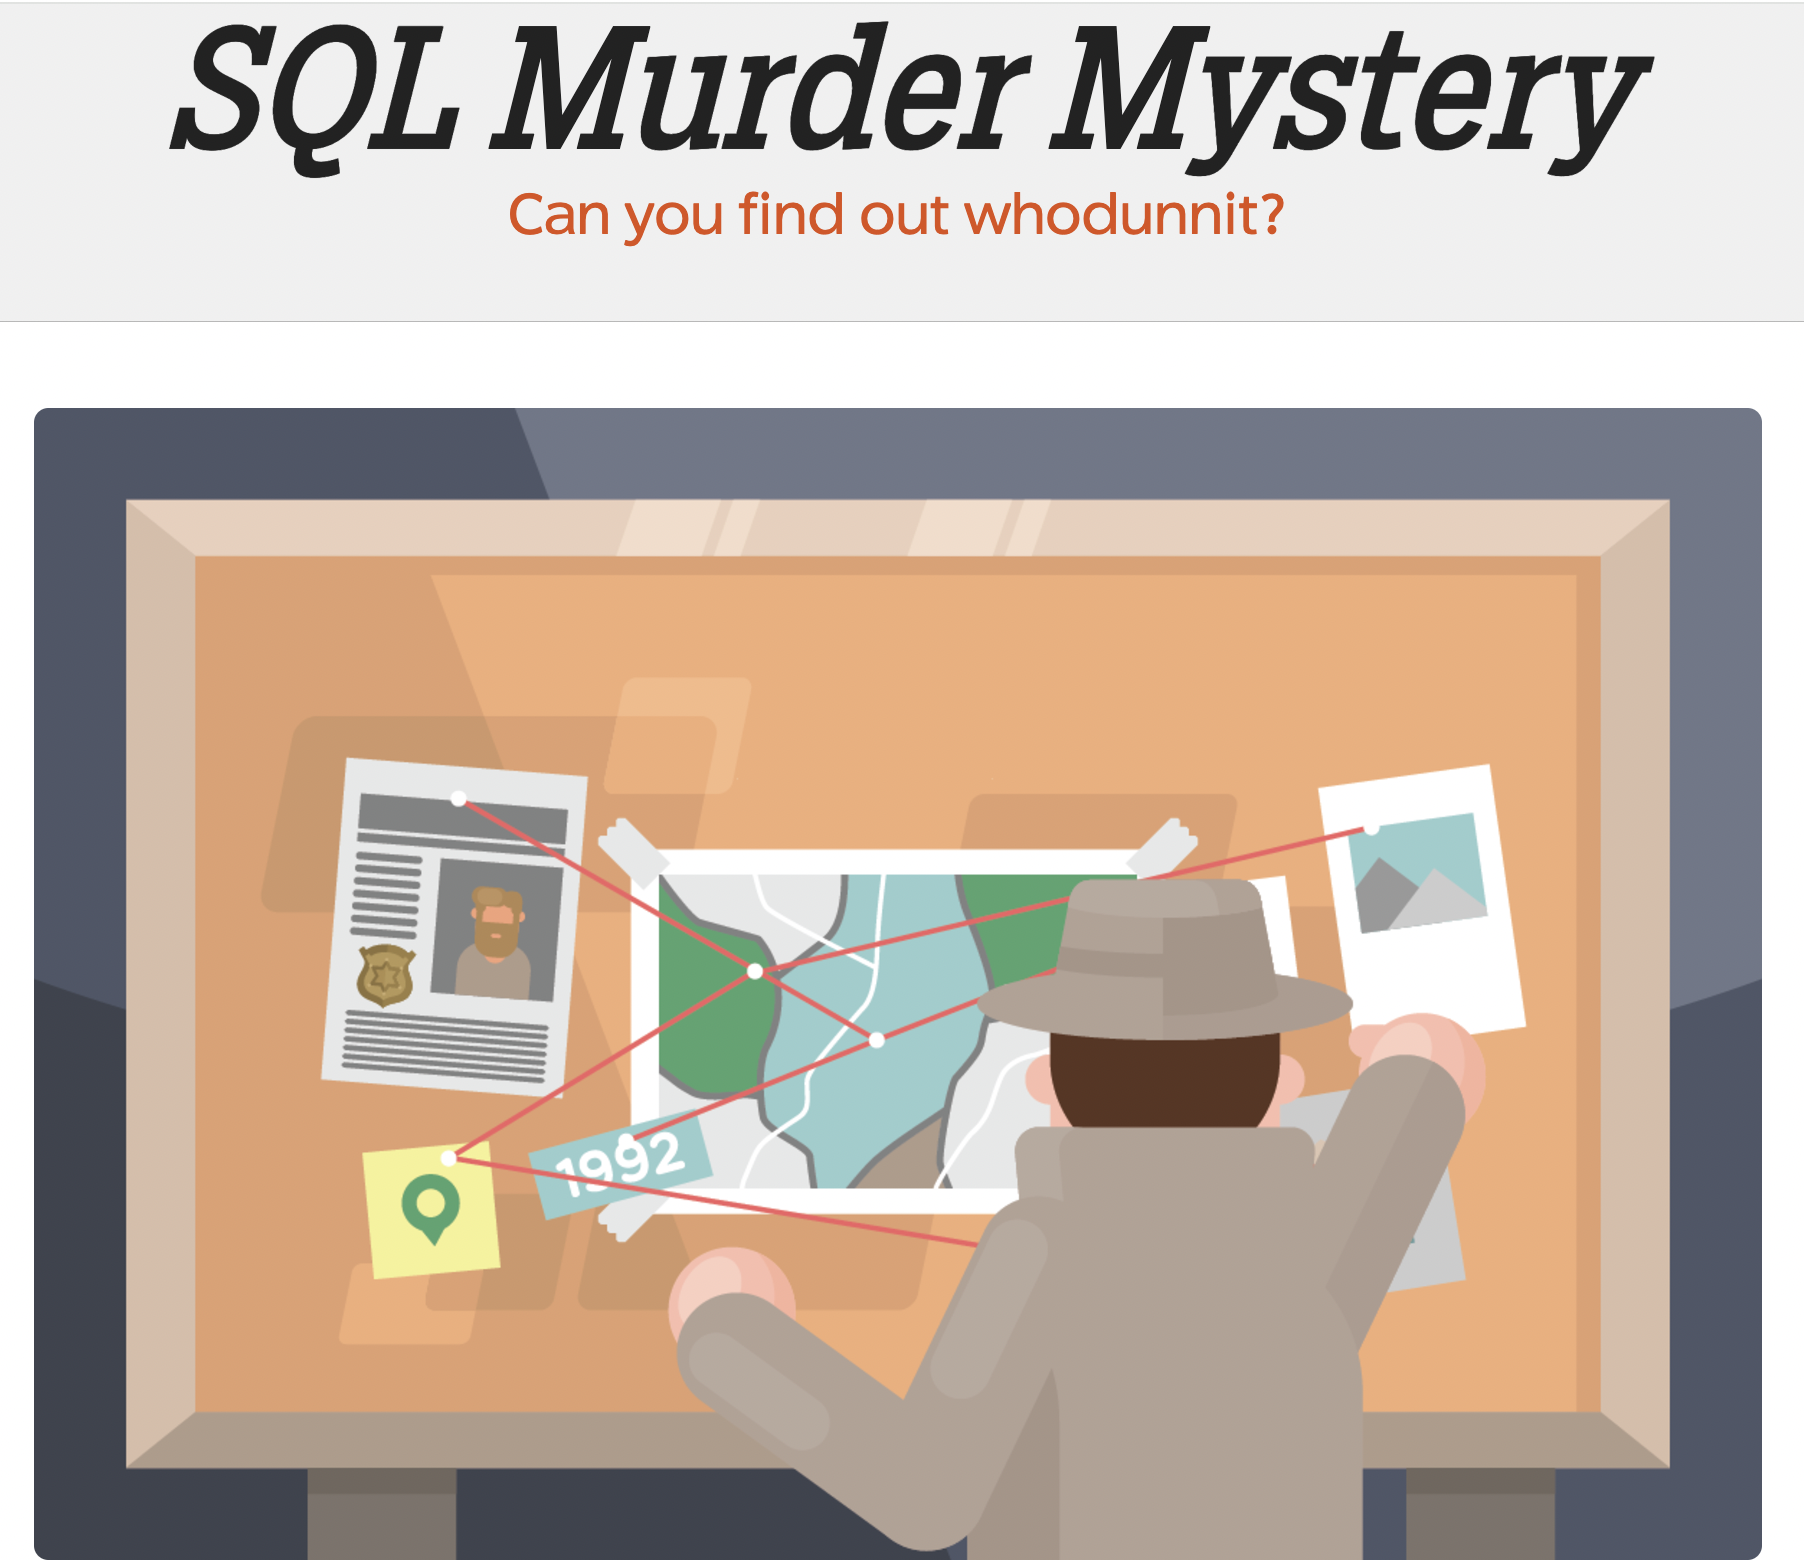
\includegraphics[width=.75\linewidth]{Images/SQL_murder.png}
  \vspace{0.5cm}
  \caption{SQL Murder Mystery}
  \label{fig:test2}
\end{minipage}
\end{figure}
\subsubsection{Bookworm Adventures}
\hspace*{1cm} Bookworm Adventures là một series game kết hợp giữa giải đố ghép chữ và yếu tố nhập vai chiến đấu. Người chơi điều khiển nhân vật chính, một chú sâu "mọt sách" Lex, trong hành trình phiêu lưu qua các thế giới thần thoại, đối đầu với quái vật và giải cứu bạn bè.\\
\hspace*{1cm} Người chơi sử dụng vốn từ vựng tiếng Anh để giúp Lex ghép các chữ cái trên màn hình thành các từ hợp lệ để tấn công quái vật bằng sức mạnh của từ ngữ. Từ càng dài và phức tạp thì sát thương gây ra càng cao.\\
\hspace*{1cm} Bookworm Adventures có hệ thống trang bị (mũ, vũ khí, phụ kiện) và dược phẩm để hỗ trợ Lex trong chiến đấu, ngoài ra còn có các chữ cái đặc biệt mang lại các hiệu ứng bổ sung (tăng sát thương, thiêu đốt, đóng băng..) khi được sử dụng để tạo từ.
\begin{figure}[H]
	\centering
	\includegraphics[width=0.75\textwidth]{Images/bookworm_play.png}
	\vspace{0.5cm}
	\caption{Tổng quan một màn chơi trong Bookworm Adventures}
\end{figure}
% \hspace*{1cm}
\subsubsection{SQL Murder Mystery}
\hspace*{1cm} SQL Murder Mystery là một trò chơi tương tác được thiết kế để giúp người chơi học và thực hành SQL thông qua việc giải quyết một vụ án bí ẩn. Chúng ta có thể chơi trực tuyến tại \def\UrlFont{\bfseries}\url{https://mystery.knightlab.com}, trò chơi hoàn toàn miễn phí và không yêu cầu cài đặt bổ sung.\\
\hspace*{1cm} Trong trò chơi, chúng ta sẽ sử dụng kĩ năng SQL của bản thân để truy bắt kẻ sát nhân đang lẫn trốn trong thành phố SQL. Trò chơi bắt đầu bằng việc khám phá một vài bảng dữ liệu, và dần dần, bạn sẽ phát hiện ra các manh mối liên quan đến vụ án mạng. Ví dụ, ngay từ đầu, bạn tìm thấy một báo cáo của cảnh sát đề cập đến hai nhân chứng nhưng không xác định được nghi phạm. Sau đó, bạn thực hiện JOIN với bảng phỏng vấn nhân chứng, và dần dần tiến gần hơn đến việc xác định tên tội phạm.
\begin{figure}[H]
	\centering
	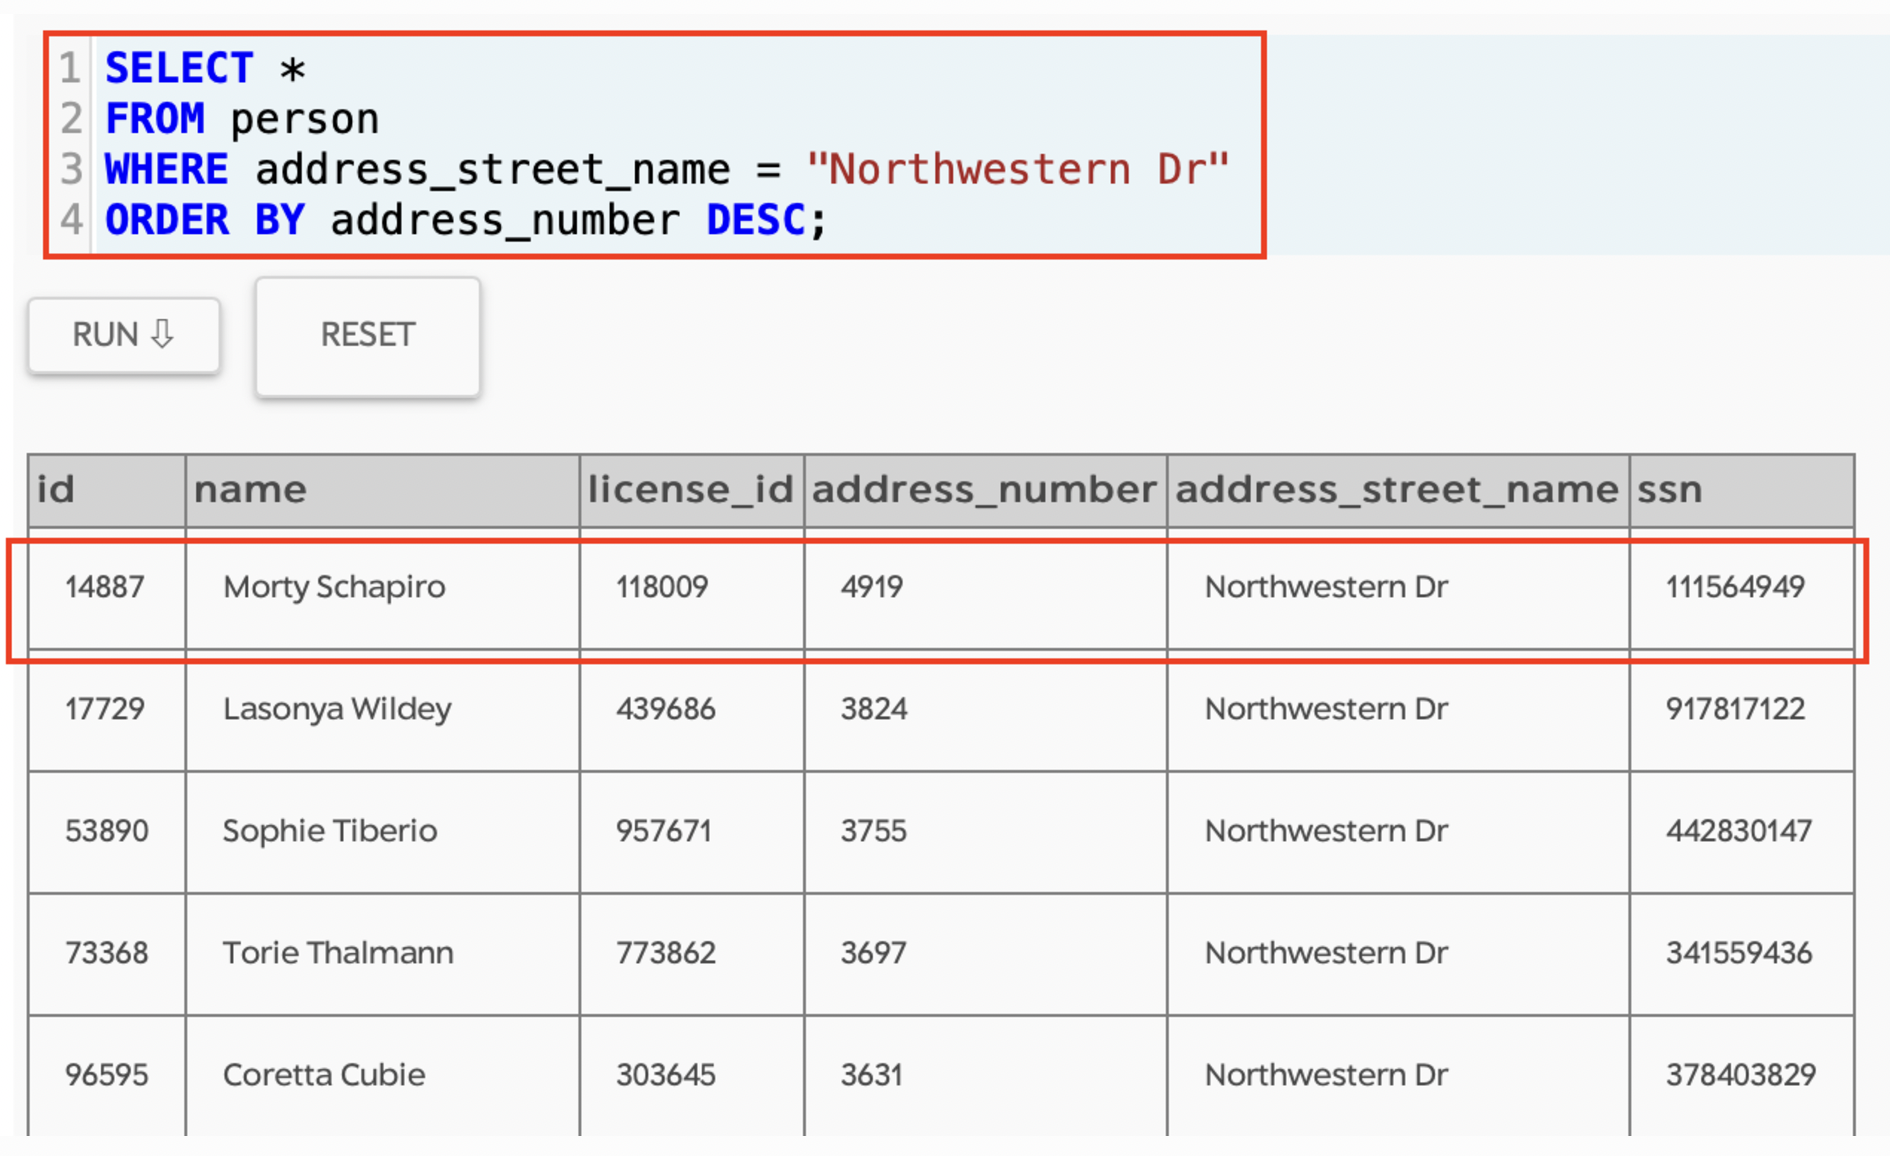
\includegraphics[width=0.75\textwidth]{Images/smm_play.png}
	\vspace{0.5cm}
	\caption{Tổng quan một câu truy vấn trong SQL Murder Mystery}
\end{figure}
\hspace*{1cm} Sau khi bắt được tên sát nhân ta nhận ra rằng hắn không phải kẻ chủ mưu thật sự. Các thám tử lại tiếp tục lên đường đi tìm tên thủ phạm đứng sau tất cả để trả lại trật tự cho thành phố SQL.
\begin{figure}[H]
\centering
\begin{minipage}{.5\textwidth}
  \centering
  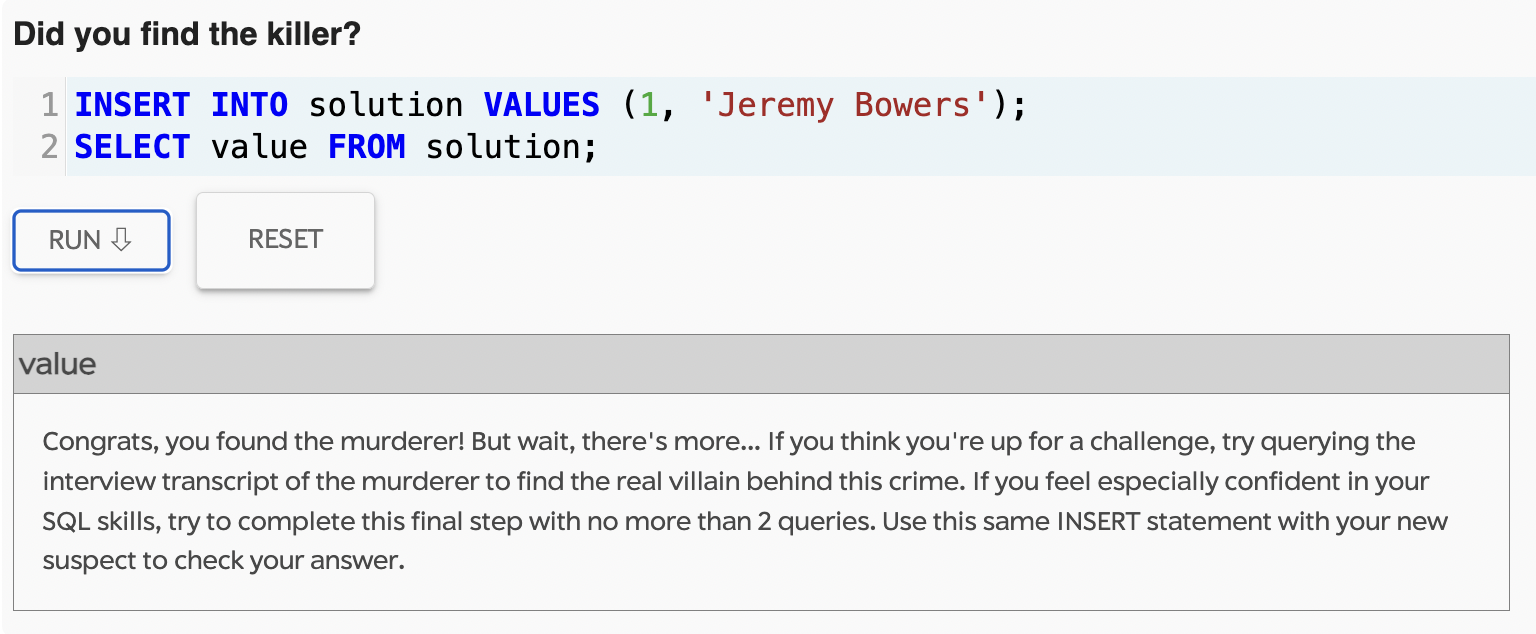
\includegraphics[width=0.75\linewidth]{Images/smm_killer.png}
  \vspace{0.5cm}
  \caption{Tìm ra kẻ sát nhân}
  \label{fig:test1}
\end{minipage}%
\begin{minipage}{.5\textwidth}
  \centering
  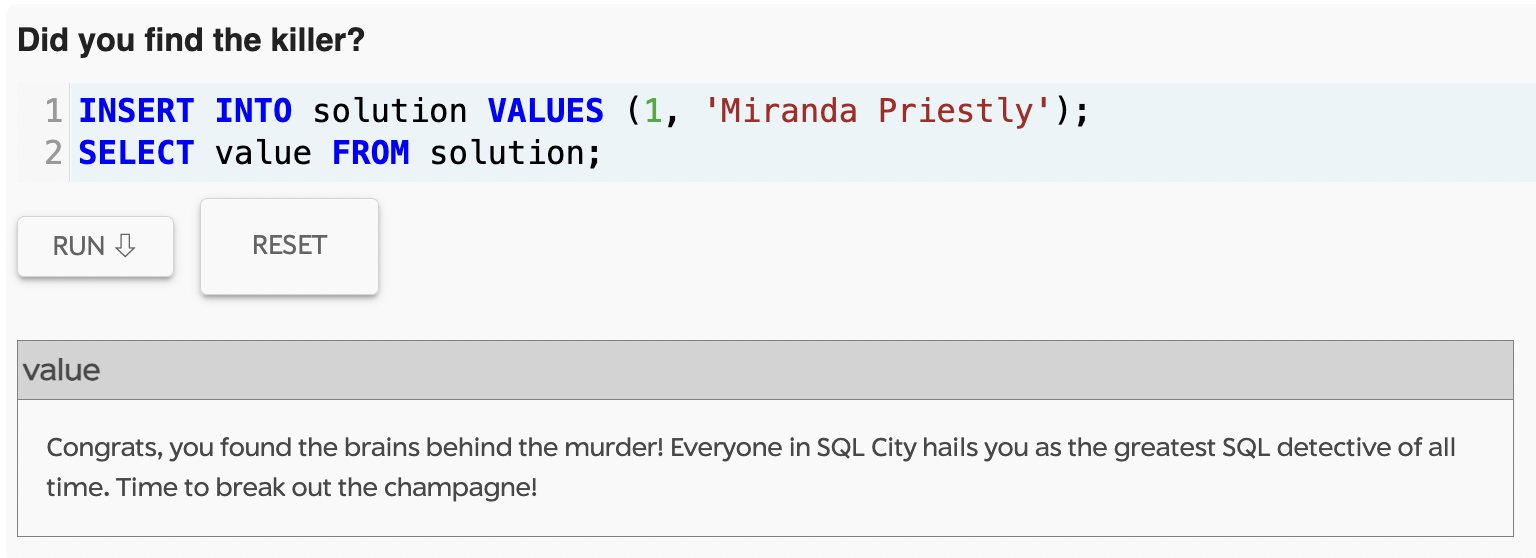
\includegraphics[width=.75\linewidth]{Images/smm_boss.png}
  \vspace{0.5cm}
  \caption{Tìm ra kẻ chủ mưu}
  \label{fig:test2}
\end{minipage}
\end{figure}
\hspace*{1cm} Trò chơi này đã nhanh chóng trở nên phổ biến nhờ cách tiếp cận sáng tạo và thú vị trong việc học lập trình SQL. Tuy nhiên, đồ hoạ của trò chơi vô cùng đơn giản, chỉ hiển thị kết quả của câu lệnh, không có hiệu ứng hay sự tương tác giữa game với người chơi. Nội dung của trò chơi cũng bị giới hạn quanh nhiềm vụ truy tìm thủ phạm, tính replay thấp.
\subsubsection{Điểm cải tiến của MeowSQL Knight}
\hspace*{1cm} Để MeowSQL Knight có thể tồn tài trên thị trường game, chúng ta cần khiến trò chơi có một nét riêng để thu hút người chơi đến với nó. Thông qua việc học tập, khắc phục những yếu điểm mà Bookworm Adventures và SQL Murder Mystery mắc phải và phát triển những tính năng mới. Trò chơi sẽ trở nên độc đáo, thu hút được một tập người chơi lớn hơn.\\
\hspace*{1cm} Đồ án kết hợp sử dụng ngôn ngữ truy vấn SQL vào chiến đấu theo lượt. Đồ án có giao diện Gameplay chính và xu hướng đồ hoạ slide scrolling giống với Bookworm Adventures. Trò chơi cũng có cốt truyện tập trung vào phiêu lưu và chiến đấu.
\subsection{Luật chơi}
\hspace*{1cm} Mỗi màn chơi, người chơi sẽ được đưa đến một bản đồ, gồm các phòng liên thông với nhau. Nhiệm vụ của người chơi là sử dụng các câu truy vấn để tương tác nhân vật chính, hoàn thành yêu cầu được đưa ra trong mỗi căn phòng, đến điểm cuối của bản đồ và hoàn thành màn chơi.

\subsection{Luật chơi Gameplay chính}
\hspace*{1cm} Mỗi màn chơi, người chơi sẽ được đưa đến một bản đồ, gồm các phòng liên thông với nhau. Nhiệm vụ của người chơi là sử dụng các câu truy vấn để tương tác nhân vật chính, hoàn thành yêu cầu được đưa ra trong mỗi căn phòng, đến điểm cuối của bản đồ và hoàn thành màn chơi.

\subsubsection{Bản đồ trong màn chơi}
\hspace*{1cm} Một màn chơi sẽ có dạng dungeon (hầm ngục) gồm nhiều phòng tại các tầng khác nhau, mỗi phòng có thể liên thông 1 chiều với nhau (có lối đi từ phòng này sang phòng khác nhưng không thể đi ngược lại) hoặc 2 chiều. Người chơi khi bắt đầu màn chơi sẽ bắt đầu ở căn phòng lối vào và kết thúc ở căn phòng lối ra. Chỉ có một lối vào và có một lối ra duy nhất. Ở lối ra thường sẽ có một Miniboss hoặc Boss trong đó. Các phòng bị bóng tối che khuất, chỉ có thể thấy các căn phòng lân cận (có lối đi từ phòng hiện tại) khi đã clear được căn phòng hiện tại.\\

\begin{figure}[H]
	\centering
	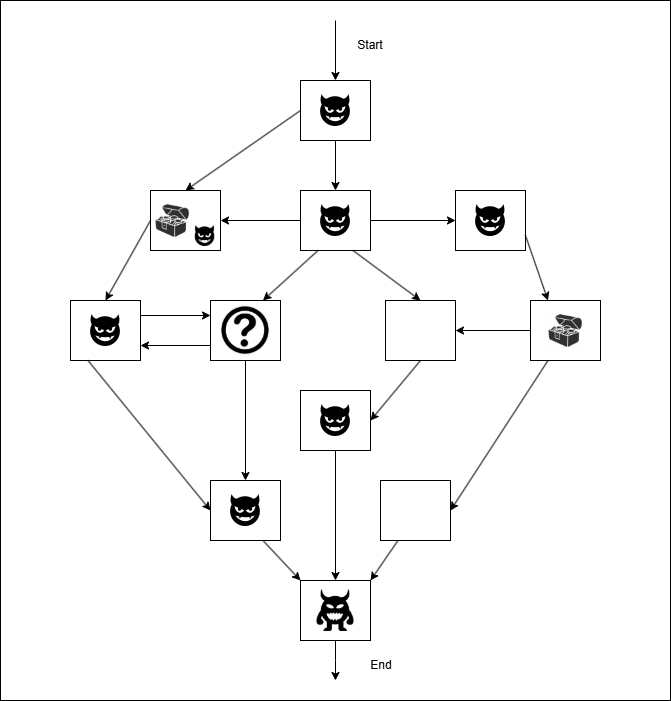
\includegraphics[width=10cm]{Images/SampleLevel.png}
	\vspace{0.5cm}
	\caption{Cấu trúc một bản đồ chơi}
\end{figure}

\hspace*{1cm}Trong một căn phòng, có thể xuất hiện quái vật, rương kho báu hoặc không có gì, đi cùng với một môi trường nhất định. Người chơi có thể chinh phục 1 căn phòng bằng các cách như tiêu diệt quái vật, mở rương kho báu hoặc đi vào 1 căn phòng trống. Sau khi chinh phục một căn phòng thì game sẽ mở khóa các căn phòng lân cận (không cần các phòng phải lối đi từ căn phòng hiện tại), người chơi quyết định đi căn phòng nào tiếp theo. Lưu ý rằng người chơi không được quay đầu (quay trở lại căn phòng đã đi trước đó). Các căn phòng có thể chứa các route đến các màn chơi khác trên bản đồ. Căn phòng cuối cùng, chính là lối ra, trong đó sẽ có một con boss hoặc min boss. Nhiệm vụ của người chơi là đánh bại boss đó để có thể thoát ra ngoài.\\
\subsubsection{Chiến đấu}
\hspace*{1cm}Gameplay chính của phần chiến đấu hoạt động theo dạng đánh theo lượt luân phiên giữa người chơi và quái vật.

\begin{itemize}
	\item Khi đến lượt của mình, người chơi được thực thi một câu lệnh hợp lệ của SQL. Câu lệnh phải chạy được thì mới tính là một câu lệnh hợp lệ. Để tấn công quái vật hoặc sử dụng vật phẩm, người chơi phải dùng câu \textbf{insert} để chèn các tham số vào các bảng mang chức năng đặc biệt. Mặc dù có cơ chế đánh theo lượt luân phiên, vẫn có khả năng người chơi sau khi xong một lượt có thể chơi một lượt nữa (đây gọi là sự nhanh nhẹn, nó sẽ là một chỉ số có ảnh hưởng đến xác suất đánh thêm lượt nữa của người chơi và quái vật). Để công bằng, cho dù người chơi có gia tăng chỉ số nhanh nhẹn cao bao nhiêu, xác suất tối đa để thêm lượt là 40\%. Điều này được tính cho cả quái vật. Tuy nhiên, mỗi thực thể chỉ có thể tấn công tối đa 2-3 lượt.
	\item Đến lượt của quái, Quái sẽ tấn công người chơi 1 lần duy nhất trong lượt, người chơi chắc chắn trúng đòn (sát thương có thể ít hay nhiều, thậm chí không đáng kể, không ảnh hưởng health). Đòn tấn công này có thể mang một số hiệu ứng khác nhau.
\end{itemize}

\subsubsection{Cơ chế đánh theo lượt}
\hspace*{1cm} Khi bắt đầu chiến đấu, lượt của thực thể được quyết định bằng một phép random với dải giá trị bao gồm điểm nhanh nhẹn của kẻ thù và người chơi, nếu random vào dải giá trị của đối tượng nào thì đối tượng đó được phép đi trước. Mỗi thực thể sẽ được cấp một chỉ số gọi là Turn Counter (TC) với giá trị ban đầu là độ nhanh nhẹn của thực thể đó. Đối với quái vật, nếu trong lượt quái vật tấn công người chơi thì TC sẽ bị giảm đi 70\% giá trị ban đầu, tương tự với player, nếu tấn công thì TC sẽ giảm 70\%, sử dụng vật phẩm thì giảm 60\%, chạy câu truy vấn hiển thị bảng ra màn hình thì giảm 60\%. Nếu TC về âm thì lượt tới sẽ là lượt của đối phương, ngược lại, việc quyết định lượt tiếp theo là của mình hay của đối phương sẽ phụ thuộc vào random tiếp với dải giá trị bao gồm TC còn lại của kẻ thù và người chơi. Nếu lượt tiếp theo là lượt của đối phương thì TC reset về chỉ số nhanh nhẹn (chưa tính trường hợp dính hiệu ứng độc, làm chậm, băng). Khi đến lượt của người chơi, nếu TC < 0 (do hiệu ứng băng) thì người chơi không thể thao tác và chuyển đến cuối lượt người chơi (nơi sẽ áp dụng hiệu ứng)\\
\subsubsection{Mã định danh thực thể}
\hspace*{1cm} Với một màn chơi, người chơi, quái vật và các bộ phận của nó sẽ được cấp một mã EntityID có cùng một định dạng, cấu trúc. Đây là chuỗi ký tự có độ dài 8 ký tự cố định (gồm số và chữ in thường và in hoa). Mỗi EntityID chỉ được sở hữu bởi nhiều nhất 1 object. Khi Object chết và màn chơi tiếp tục, EntityID này sẽ được thu hồi và nó không còn tồn tại với bất kỳ hình thức nào. Có một bảng lưu trữ các EntityID và loại Object được cấp phát.
\subsubsection{Người chơi}
\hspace*{1cm} Người chơi sẽ có một bảng trong schema để lưu trữ các thông tin khác nhau cần thiết cho việc chiến đấu với entityID thuộc về người chơi, các thuộc tính của người chơi tương tự với các Game RPG.\\
\begin{itemize}
	\item \textbf{Máu tối đa của người chơi} (base + current)
	\item \textbf{Máu hiện tại của người chơi}
	\item \textbf{Mô tả người chơi}
	\item \textbf{Màu sắc người chơi} (optional)
	\item \textbf{Sát thương cơ bản của người chơi} (base)
	\item \textbf{Nhanh nhẹn cơ bản}
	\item \textbf{Giáp của người chơi} (base + current)
	\item \textbf{Max slot trang bị}
	\item \textbf{EntityID của người chơi}
	\item \textbf{Level của người chơi}, có ảnh hưởng đến các chỉ số khác của người chơi, đồng thời ảnh hưởng khả năng sử dụng trang bị (giảm hoặc tăng)
\end{itemize}

\hspace*{1cm} Ngoài ra, người chơi được cung cấp một số lượng slot trang bị nhất định, người chơi trang bị vũ khí và giáp vào các slot này, mỗi slot chỉ được chứa một trang bị. Người chơi sẽ có môt inventory để chứa các vật phẩm và các trang bị không sử dụng. Trong chiến đấu, các vật phẩm tiêu hao sẽ được highlight và người chơi chỉ có thể được sử dụng chúng trong chiến đấu.
\subsubsection{Quái vật}
\hspace*{1cm} Mỗi quái vật có thông tin được lưu trữ trong 1 row của bảng Monster trong Schema. Các quái vật vẫn mang các chỉ số thuộc tính tương tự người chơi, tuy nhiên nó không có điểm máu (HP), vì vậy nó không tồn tại nhờ HP. Một số thuộc tính cơ bản:\\
\begin{itemize}
	\item \textbf{Tên quái vật}
	\item \textbf{Độ trà trộn}
	\begin{itemize}
		\item Thuộc tính trà trộn vào bảng thực thể và bảng monster.
		\item Một monster có thể có các bản sao làm hình nộm của nó và sẽ mang các EntityID riêng, chủ yếu để người chơi khó xác định được đâu mới là con thật mà tấn công (có thể gộp chung vào trí thông minh).
	\end{itemize}
	\item \textbf{Giáp cơ bản}: Bao gồm giáp và kháng hiệu ứng.
	\item \textbf{Màu sắc thân của quái vật}
	\item \textbf{Chủng loại quái vật}
	\item \textbf{Sát thương cơ bản: } Bao gồm sát thương thường, sát thương chí mạng và sát thương hiệu ứng
	\item \textbf{Nhanh nhẹn}
	\item \textbf{Nguồn gốc xuất xứ của quái vật}
	\item \textbf{Level}
	\item \textbf{Mô tả sơ bộ}
	\item \textbf{Phẩm chất (Traits):} mỗi quái vật sẽ có một phẩm chất, chủ yếu để chịu tác động từ môi trường.
\end{itemize}
\hspace*{1cm} Ngoài ra còn có các bảng liên quan đến Monster nhằm cung cấp gợi ý cho người chơi để xác định Entity của quái vật đúng.
\hspace*{1cm} Như đã nói ở trên, quái sẽ không sống nhờ HP, mà chúng sẽ sống nhờ vào các bộ phận chí mạng trên cơ thể, Tình trạng sống/chết của quái vật phụ thuộc vào tình trạng tồn tại của các bộ phận này. Nếu mất hết tất cả bộ phận chí mạng, quái sẽ chết. Quái cũng sẽ có một bộ kỹ năng, nhất định. Khi đến lượt của quái, quái sẽ chọn ngẫu nhiên một kỹ năng đã sẵn sàng và thi triển, kỹ năng nó cũng sẽ mất một khoảng thời gian để phục hồi. Các kỹ năng có đều mang một trait liên quan đến trait của bộ phận chí mạng. Nếu không có kỹ năng nào sẵn sàng để sử dụng, quái vật sẽ bỏ qua đợt tấn công.\\
\hspace*{1cm} Các bộ phận có thể nằm rải rác trên cơ thể và có EntityID tương tự với Quái vật và người chơi. Thông tin một bộ phận sẽ là một bảng ghi của bảng Monster Part chứa thông tin chung của tất cả bộ phận quái vật, bao gồm cả bộ phận ảo - bộ phận ngụy trang,… trong một level) trong Schema. Quái vật có thể có một số lượng bộ phận nhất định. Khi người chơi tấn công vào các bộ phận này, nếu nó không có chủ (hoặc chủ đã chết) sẽ được tính sát thương cao nhất (chưa trừ cộng về mặt khắc chế hoặc áp chế), ngược lại sẽ phải chịu giáp và kháng hiệu ứng của quái vật, rồi mới trừ vào máu của bộ phận, hiệu ứng sẽ áp dụng cho quái vật, người chơi vẫn tấn công vào EntityID của quái vật bình thường, nhưng hoàn toàn vô dụng, cả sát thương và hiệu ứng đều sẽ không áp dụng cho quái vật. Một số đặc điểm của một bộ phận. \\
\begin{itemize}
	\item \textbf{Máu tối đa}
	\item \textbf{Máu hiện tại}
	\item \textbf{Độ trà trộn}
	\begin{itemize}
		\item Thuộc tính trà trộn vào bảng thực thể và bảng Monster Part.
		\item Một monster có thể có các bản sao bộ phận làm hình nộm của nó và sẽ mang các EntityID riêng, chủ yếu để người chơi khó xác định được đâu mới là con thật mà tấn công. Chúng sử dụng trí thông minh để trà trộn các bộ phận ảo này vào. Các bộ phận này sẽ có máu bằng máu của bộ phận thật, tuy nhiên khi tấn công sẽ có xác suất 40\% bị huỷ diệt khi nhận sát thương. Một số bộ phận giả có thể đi kèm các hiệu ứng bẫy khi người chơi tiêu diệt các bộ phận này.
	\end{itemize}
	\item \textbf{Loại bộ phận} (tay súng, tay dao,…)
	\item \textbf{Phẩm chất (Traits):} mỗi bộ phận sẽ có tối đa 2 phẩm chất.
	\item \textbf{Nguồn gốc xuất xứ của quái vật}
	\item \textbf{Mô tả sơ bộ}
\end{itemize}
\hspace*{1cm} Ngoài ra còn có các bảng liên quan đến Monster Part (thường sẽ chung các bảng với Monster) nhằm cung cấp gợi ý cho người chơi để xác định Entity của quái vật đúng. Để có thể xác định EntityID chính xác, người chơi cần dựa vào tiếng kêu, các đặc điểm bề ngoài cũng như phản ứng đòn đánh và khi bị đánh của quái vật để nhận biết.
\hspace*{1cm} Quái sẽ tạo các bản sao Monster và Monster Part dựa trên độ trà trộn, độ trà trộn có thể ảnh hưởng đến số bản sao Monster, số bản sao Monster Part và độ giống với bản gốc (độ trà trộn càng cao thì record bản sao càng có xác suất giống bản gốc cao). Người chơi cần chú ý chỉ số này để có thể đưa ra các quyết định hợp lý.
\subsubsection{Hiệu ứng}
\begin{itemize}
	\item \textbf{Độc}
	\begin{itemize}
		\item Gây sát thương: 5\% lượng máu tối đa khi hết lượt
		\item Giảm độ nhanh nhẹn: 40\%
	\end{itemize}
	\item \textbf{Lửa}
	\begin{itemize}
		\item Gây sát thương: 15\% lượng máu tối đa khi hết lượt
	\end{itemize}
	\item \textbf{Băng}
	\begin{itemize}
		\item Giảm độ nhanh nhẹn xuống -1\%
	\end{itemize}
	\item \textbf{Làm chậm}
	\begin{itemize}
		\item Giảm độ nhanh nhẹn xuống 50\%
	\end{itemize}
	\item \textbf{Hiệu ứng câu lệnh}
	\begin{itemize}
		\item Người chơi không được sử dụng một từ khóa nhất định trong câu lệnh
	\end{itemize}
	\item \textbf{Mù}
	\begin{itemize}
		\item Người chơi sẽ không nhìn được một số ô trong bảng với câu \texttt{SELECT}
	\end{itemize}
\end{itemize}

\textbf{Chỉ số kháng hiệu ứng}
\begin{itemize}
	\item Mỗi người chơi/quái vật sẽ có một bộ chỉ số kháng hiệu ứng nhất định.
	\item Khi tấn công đối phương, nếu kháng hiệu ứng tương ứng lớn hơn sát lực hiệu ứng, đối phương sẽ không dính hiệu ứng.
	\item Nếu kháng hiệu ứng nhỏ hơn sát lực hiệu ứng, đối phương sẽ chịu hiệu ứng với trạng thái (state) của hiệu ứng cộng thêm sát lực hiệu ứng đó trừ cho kháng hiệu ứng.
	\item Trước khi kết thúc lượt của đối tượng hiện tại, hiệu ứng sẽ gây sát thương (nếu có) và trạng thái hiệu ứng được trừ đi một lượng chỉ số bằng kháng hiệu ứng của người chơi. Nếu trạng thái hiệu ứng nhỏ hơn hoặc bằng 0, hiệu ứng sẽ kết thúc.
\end{itemize}

\textbf{Trang bị và sát lực hiệu ứng}
\begin{itemize}
	\item Chỉ số kháng hiệu ứng của người chơi được tổng hợp từ nhiều trang bị trong slot.
	\item Mỗi món trang bị sẽ có một bộ sát lực riêng và không tính tổng hợp.
	\item Khi người chơi tấn công bộ phận nào của quái vật, sẽ tính sát lực hiệu ứng trên món trang bị và kỹ năng (skill) được sử dụng để tấn công.
\end{itemize}

\textbf{Hiệu ứng trên quái vật}
\begin{itemize}
	\item Quái vật sẽ chịu hiệu ứng trên thực thể của quái vật.
	\item Hiệu ứng sẽ gây sát thương lên bộ phận đó của quái vật.
\end{itemize}

\subsubsection{Trait System}
\hspace*{1cm} Có một bộ các Trait (phẩm chất) được sử dụng chung bởi các thực thể và trang bị. Mỗi object nói trên sẽ có một số lượng trait nhất định.\\
\hspace*{1cm} Trong hệ thống trait, Một trait có thể bị một hoặc nhiều trait khác khắc chế, hoặc một trait trait có thể khắc chế nhiều trait khác, cũng có thể không bị khắc chế hay khắc chế trait nào. Số lượng trait khắc chế không được vượt quá một ngưỡng nào đó. Hệ thống trait sẽ luôn được điều chỉnh bởi người thiết kế màn chơi, người thiết kế phải cố gắng giữ cho các trait được cân bằng, không có trait nào quá mạnh, quá yếu.\\ 
\hspace*{1cm} Quái vật sẽ có 1 trait, chịu khắc chế của môi trường (bản thân môi trường cũng có một trait, chủ yếu gây khắc chế và áp chế) ảnh hưởng đến đòn đánh, Bộ phận của quái cũng có tối đa 2 trait, chịu khắc và áp chế từ sát thương vũ khí người chơi.
\subsubsection{Cơ chế kho đồ/trang bị}
Thứ cần thiết cho game không thể thiếu là các vật phẩm, các trang bị sẽ hỗ trợ người chơi trên chuyến hành trình. Các vật phẩm có thể có nhiều cách thu thập khác nhau:
\begin{itemize}
	\item Thu thập khi mở rương trong màn chơi
	\item Thu thập qua đánh boss
	\item Mua bán, trao đổi
	\item Gacha
	\item Ghép vật phẩm
\end{itemize}

Các vật phẩm sẽ có các thuộc tính khác nhau, và có các công dụng khác nhau giúp người chơi có thể lựa chọn.

\textbf{Phân cấp theo độ hiếm}
Việc phân cấp này chủ yếu diễn ra ở trang bị, có thể chia thành các phân cấp như sau:
\begin{itemize}
	\item Common
	\item Uncommon
	\item Rare
	\item Super-Rare
	\item Myth
	\item Legendary
\end{itemize}

Mỗi phân cấp khác nhau sẽ mở khóa tiềm năng trang bị khác nhau, bao gồm chỉ số cơ bản, giới hạn chỉ số tối đa, các skill độc quyền,...

Đối với các item tiêu thụ được, kích thước của chúng phụ thuộc vào 3 độ hiếm: 
\begin{itemize}
	\item Common (nhỏ)
	\item Uncommon (vừa)
	\item Rare (lớn)
\end{itemize}
Độ hiếm càng cao giới hạn chỉ số càng lớn, ngoài ra còn đi kèm các hiệu ứng mạnh hơn, cũng như nhiều traits hơn (giới hạn tối đa 5 traits)
\textbf{Các chỉ số trang bị}
Trang bị vũ khí và trang bị giáp đều mang một bộ chỉ số cố định, phù hợp cho việc hiện thực cũng như cho việc khi combat, người chơi có thể sử dụng giáp để chiến đấu.
\begin{itemize}
	\item Chỉ số cơ bản
	\item Phẩm chất (Traits)
	\begin{itemize}
		\item tấn công cơ bản
		\item giáp cơ bản
		\item nhanh nhẹn
		\item kháng hiệu ứng
		\item hút máu
		\item phản đòn
		\item hồi máu mỗi lượt
		\item ...
	\end{itemize}
	\item Giới hạn chỉ số
	\begin{itemize}
		\item tấn công tối đa
		\item giáp tối đa
		\item kháng hiệu ứng tối đa
	\end{itemize}
	\item Nâng cấp
	\begin{itemize}
		\item Hệ số nâng cấp giáp
		\item Hệ số nâng cấp vũ khí
	\end{itemize}
	\item Ảnh hưởng của Level người chơi
	\begin{itemize}
		\item Level yêu cầu
		\item Mức giảm stat nếu dưới level
	\end{itemize}
\end{itemize}

\textbf{Các loại trang bị}
\begin{itemize}
	\item Vũ khí
	\begin{itemize}
		\item Vũ khí dùng để tấn công quái vật cho ra sát thương tốt nhất, mỗi loại vũ khí khác nhau sẽ có bộ kỹ năng khác nhau.
	\end{itemize}
	\item Giáp
	\begin{itemize}
		\item Khi quái vật tấn công vào giáp thì giáp sẽ phát huy hiệu quả khi ngăn cản đòn đánh của quái vật cũng như có thể kháng hiệu ứng. Người chơi vẫn có thể tấn công quái vật bằng giáp được, nhưng sát thương của chúng thường rất nhỏ.
	\end{itemize}
	\item Giày
	\begin{itemize}
		\item Giày có thể tăng chỉ số giáp và nhanh nhẹn, cũng như giáp, chỉ số tấn công gần như bằng 0 nên Khi quái vật tấn công vào thì giáp sẽ phát huy hiệu quả khi ngăn cản đòn đánh của quái vật cũng như có thể kháng hiệu ứng.
	\end{itemize}
	\item Kỹ năng (Chiêu)
	\begin{itemize}
		\item Mỗi món trang bị có một chiêu nhất định, giúp khuếch đại đòn đánh cũng như đi kèm với các hiệu ứng khác nhau, chủ yếu là lửa, độc, băng,...
		\item Một số thông số của chiêu cơ bản:
		\begin{itemize}
			\item Hệ số khuếch đại sát thương
			\item Hệ số khuếch đại giáp cơ bản
			\item Hệ số khuếch đại nhanh nhẹn
			\item Hệ số hút máu
			\item ...
		\end{itemize}
	\end{itemize}
	\item Khi sử dụng vũ khí có trait tấn công bộ phận quái vật, ta sẽ xét tổng số cặp khắc chế và tổng số cặp bị khắc chế của vũ khí sử dụng. Nếu số cặp khắc chế lớn hơn thì xem như đòn đánh có lợi thế về khắc chế.
	\item Về giáp và giày có nhiều trait, trait tổng quan của player được tính là hợp của tập các trait của từng trang bị. Nếu số trait lớn hơn 5, thì trang bị đứng trước sẽ được ưu tiên về trait hơn.
\end{itemize}
\textbf{Cơ chế Kho đồ/ Slot trang bị}
\begin{itemize}
	\item Kho đồ trong game có không gian lưu trữ lớn, nhưng nó có giới hạn, chủ yếu lưu trữ các trang bị không sử dụng và các vật phẩm tiêu hao cùng vật phẩm khác. Khi người chơi chết thì tất cả các món đồ trong kho không bị ảnh hưởng.
	\item Slot trang bị cho phép người chơi gán các trang bị vào để mang đi chiến đấu. Có tối đa 8 slot trang bị, ban đầu người chơi chỉ có 4 slot trang bị, có thể nâng cấp tại cửa hàng. Nếu người chơi chết, các món trang bị không bị mất, nhưng chúng sẽ bị giảm cấp độ (tùy dev tùy chỉnh mà có thể giảm ít, hay nhiều).
	\item Trong màn chơi, người chơi không được gán trang bị từ kho vào slot và ngược lại. Việc này chỉ được thực hiện bên ngoài bản đồ hay ở khu Safe Zone.
\end{itemize}
\subsubsection{Môi trường}
\textbf{1cm} Mỗi căn phòng trong màn chơi có một môi trường tương ứng. Có một bảng gồm ID phòng, một mã môi trường trong căn phòng đó, cùng với thuộc tính (trait) của môi trường. Các vật phẩm, quái vật sẽ chịu ảnh hưởng của môi trường theo hướng mạnh hơn, yếu đi hoặc không bị ảnh hưởng tương ứng với mã môi trường. Mã môi trường là cố định.\\

\textbf{Vật thể trong môi trường}
\textbf{1cm} Ngoài ID môi trường trong phòng, mỗi phòng sẽ có một bảng tên là Environment Object chỉ các vật thể trong môi trường. Các vật thể sử dụng EntityID làm khóa chính tương tự với các object khác. Ngoài ra còn có mô tả được sinh bởi hệ thống game, giúp người chơi thu thập các manh mối tạo lợi thế trong màn chơi. Bảng này người chơi có thể thêm và xóa các record khác nhau. Tuy nhiên, cần cẩn thận vì một số vật thể nếu xóa đi sẽ gây bất lợi cho người chơi, thậm chí còn có thể giết người chơi ngay lập tức.\\

\hspace*{1cm} Các vật thể này có thể được sử dụng làm vũ khí để tấn công, nếu nó được xem là có thể gây sát thương (ví dụ như dao từ quái vật phi dao). Nếu không, khi tấn công, game sẽ thông báo rằng object người chơi chọn để tấn công không có gì xảy ra sau đó.\\

\subsubsection{Cơ chế gõ lệnh}
\hspace*{1cm}Người chơi chỉ được gõ lệnh khi đến lượt của mình, Ngôn ngữ truy vấn người chơi sử dụng là SQL, thuộc dạng Declarative Language. Người chơi chỉ được thực hiện 1 câu lệnh, nếu người chơi cố tình nhập nhiều câu lệnh trong một lượt thì game sẽ thực thi câu lệnh đầu tiên được nhập vào và hủy toàn bộ các câu lệnh sau (đồng thời nhắc nhở người chơi về hành động này).\\
\hspace*{1cm} Người chơi có thể sử dụng các câu truy vấn \texttt{SELECT} để lấy thông tin của một bảng trong schema, một bảng người chơi tự tạo,... Người chơi có thể chèn giá trị, cập nhật giá trị và xóa giá trị cho bảng đó cho mục đích khác nhau.\\
\hspace*{1cm} Người chơi sử dụng schema để xác định EntityID phù hợp để tấn công. Muốn tấn công quái vật người chơi cần chèn vào bảng Attack với các giá trị 
\begin{verbatim}
	(EntityID target, ItemID equipment, [optional] SkillID skill)
\end{verbatim}
Trong đó:
\begin{itemize}
	\item \textbf{target}: EntityID mục tiêu cần tấn công, mục tiêu có thể là của quái vật, của bộ phận và cả của người chơi.
	\item \textbf{equipment}: ID trang bị sử dụng để tấn công (vấn đề này sẽ được nói trong phần sau), ID này phải là của item nằm trong slot trang bị. Trang bị tấn công có thể là giáp và vũ khí.
	\item \textbf{skill}: là mã của chiêu thức tương ứng với vũ khí, (có thể thay bằng index cho tiện). Mỗi trang bị sẽ có một số chiêu thức nhất định, người chơi có thể lựa chọn chiêu thức, cũng như tham khảo chúng từ bảng trong schema. Người chơi có thể tấn công bằng đánh thường (không nhập index chiêu).
\end{itemize}

Ngoài ra, người chơi có thể sử dụng các vật phẩm tiêu hao để hỗ trợ trong chiến đấu bằng cách chèn giá trị vào bảng Use với giá trị:
\begin{verbatim}
	(ItemID item)
\end{verbatim}
trong đó \texttt{item} là vật phẩm tiêu hao được trong inventory, các item này sẽ hiện lên đầu tab Inventory và sẽ được highlight để người chơi nhận biết.
\subsubsection{Win condition}
Người chơi sẽ thắng khi đánh bại được quát vật, tức là khiến cho hp của nó về 0.
\subsubsection{Lose condition}
Người chơi sẽ thua khi bị tiêu diệt bởi quái vật, để hp của mình chạm đến 0.
\subsection{Các đối tượng chính trong màn chơi}
\subsubsection{Người chơi}
\begin{figure}[H]
	\centering
	
\includegraphics[width=5cm]{Images/Player.png}
	\vspace{0.5cm}
	\caption{Người chơi}
\end{figure}
\subsubsection{Quái vật}
\begin{figure}[H]
	\centering
	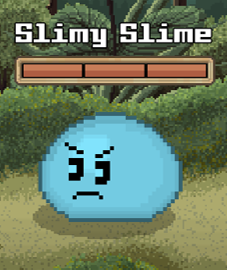
\includegraphics[width=5cm]{Images/Monster.png}
	\vspace{0.5cm}
	\caption{Quái vật}
\end{figure}
\subsubsection{Thông số, trang bị và kho đồ}
\begin{figure}[H]
	\centering
	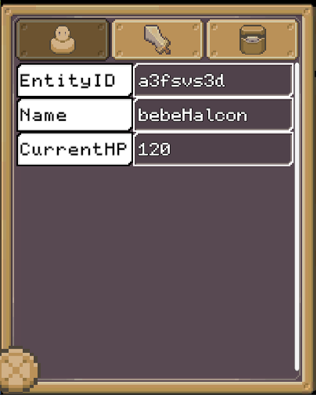
\includegraphics[width=10cm]{Images/Inventory.png}
	\vspace{0.5cm}
	\caption{Thông số, trang bị và kho đồ}
\end{figure}
\subsubsection{Ô nhập lệnh và kết quả truy vấn}
\begin{figure}[H]
	\centering
	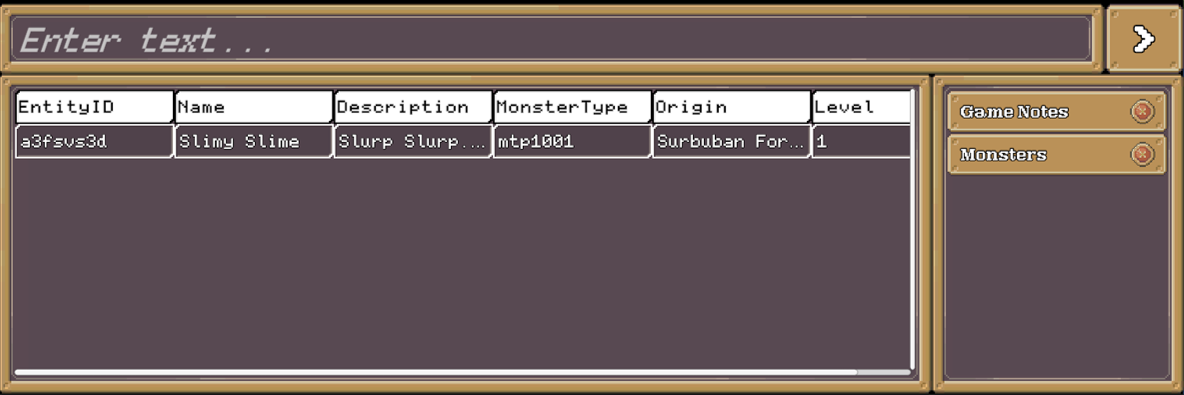
\includegraphics[width=10cm]{Images/CommandBox.png}
	\vspace{0.5cm}
	\caption{Ô nhập lệnh và kết quả truy vấn}
\end{figure}
\subsubsection{Bản đồ màn chơi và phòng hiện tại}
\begin{figure}[H]
	\centering
	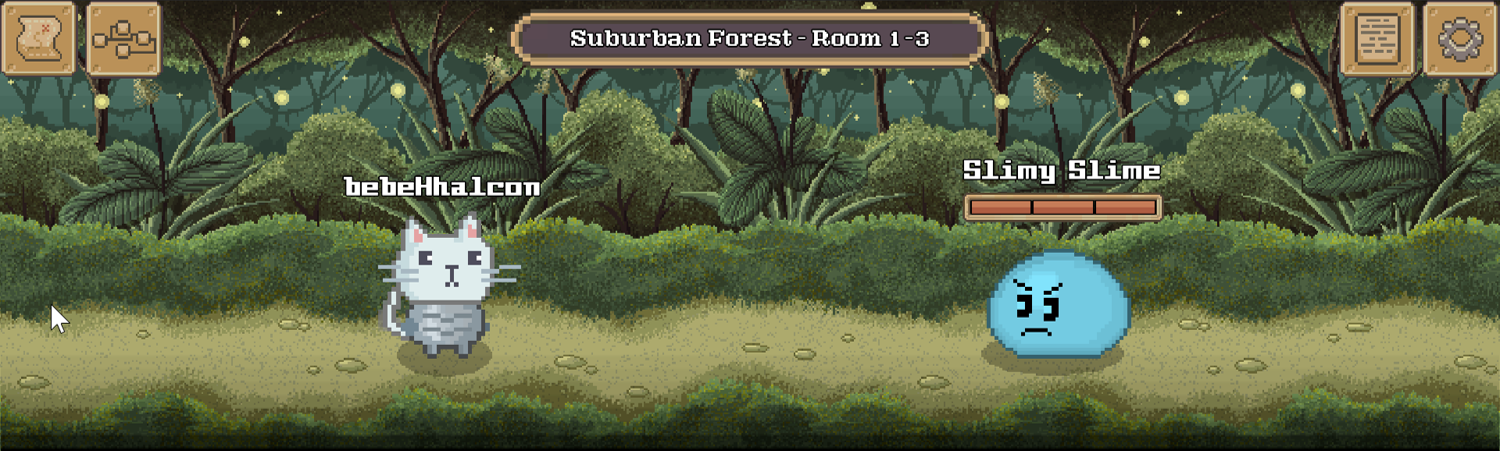
\includegraphics[width=10cm]{Images/CurrentRoom.png}
	\vspace{0.5cm}
	\caption{Quang cảnh môi trường của phòng chơi hiện tại}
\end{figure}
